\documentclass[11pt,a4paper]{article}
\usepackage[margin=2.3cm]{geometry}
\usepackage{graphicx,amsmath,xcolor,enumitem,booktabs,caption}
\usepackage[version=4]{mhchem}
\usepackage[most]{tcolorbox}
\usepackage[hidelinks]{hyperref}
\graphicspath{{figures/}}
\setlist{itemsep=2pt,topsep=3pt}
\setlength{\parindent}{0pt}
\setlength{\parskip}{5pt}

% ---- my note boxes ----------------------------------------------------------
\newtcolorbox{aha}{colback=green!5,colframe=green!45!black,boxrule=0.5pt,arc=2pt,
  left=5pt,right=5pt,top=3pt,bottom=3pt,fonttitle=\bfseries\small,title=Aha}
\newtcolorbox{oops}{colback=red!4,colframe=red!55!black,boxrule=0.5pt,arc=2pt,
  left=5pt,right=5pt,top=3pt,bottom=3pt,fonttitle=\bfseries\small,title=Mistake I caught}
\newtcolorbox{askme}{colback=yellow!8,colframe=orange!70!black,boxrule=0.5pt,arc=2pt,
  left=5pt,right=5pt,top=3pt,bottom=3pt,fonttitle=\bfseries\small,title=Test myself}
\newcommand{\q}[1]{\par\textbf{Q: #1}\par}
\newcommand{\remember}[1]{\par\colorbox{blue!8}{\parbox{\dimexpr\linewidth-2\fboxsep}{\small\textbf{Remember:} #1}}\par}

\begin{document}

{\Large\bfseries Learning notes: visualising molecules}\\[2pt]
{\small photocatalyst-dft, week 1 \quad|\quad Oct 2026 \quad|\quad tools: RDKit, py3Dmol, PySCF (+ Claude / Claude Science for coding)}

\hrule\vspace{6pt}

\textbf{Why I'm writing this.} I can now make nice pictures of molecules, but the point of these
notes is to write down \emph{why} each picture exists and what it fooled me with. One sentence to
remember:

\remember{every picture answers one question, and should come with a number. Otherwise I'm just
looking at what the isovalue / viewing angle / colours decided to show me.}

My mental map so far:
\begin{itemize}
  \item \textbf{2D} (RDKit, from SMILES) $\to$ ``is this the right molecule and charge?''
  \item \textbf{3D} (py3Dmol, from xyz) $\to$ ``is the shape sensible: flat, twisted, crowded?''
  \item \textbf{overlay} (two xyz files) $\to$ ``how much did DFT move the force-field structure?''
  \item \textbf{orbitals} (PySCF $\to$ cube file $\to$ viewer) $\to$ ``where does the electron leave from / go to?''
\end{itemize}

%=============================================================================
\section*{1. 2D pictures: checking what I typed}

\q{Why bother drawing a 2D picture if I'm going to do 3D anyway?}
Because it's the cheapest check there is, and it catches the most expensive mistakes. A SMILES
with a missing bromine or the wrong charge still runs. DFT will happily spend hours on a molecule
that doesn't exist.

\begin{figure}[h]
\centering
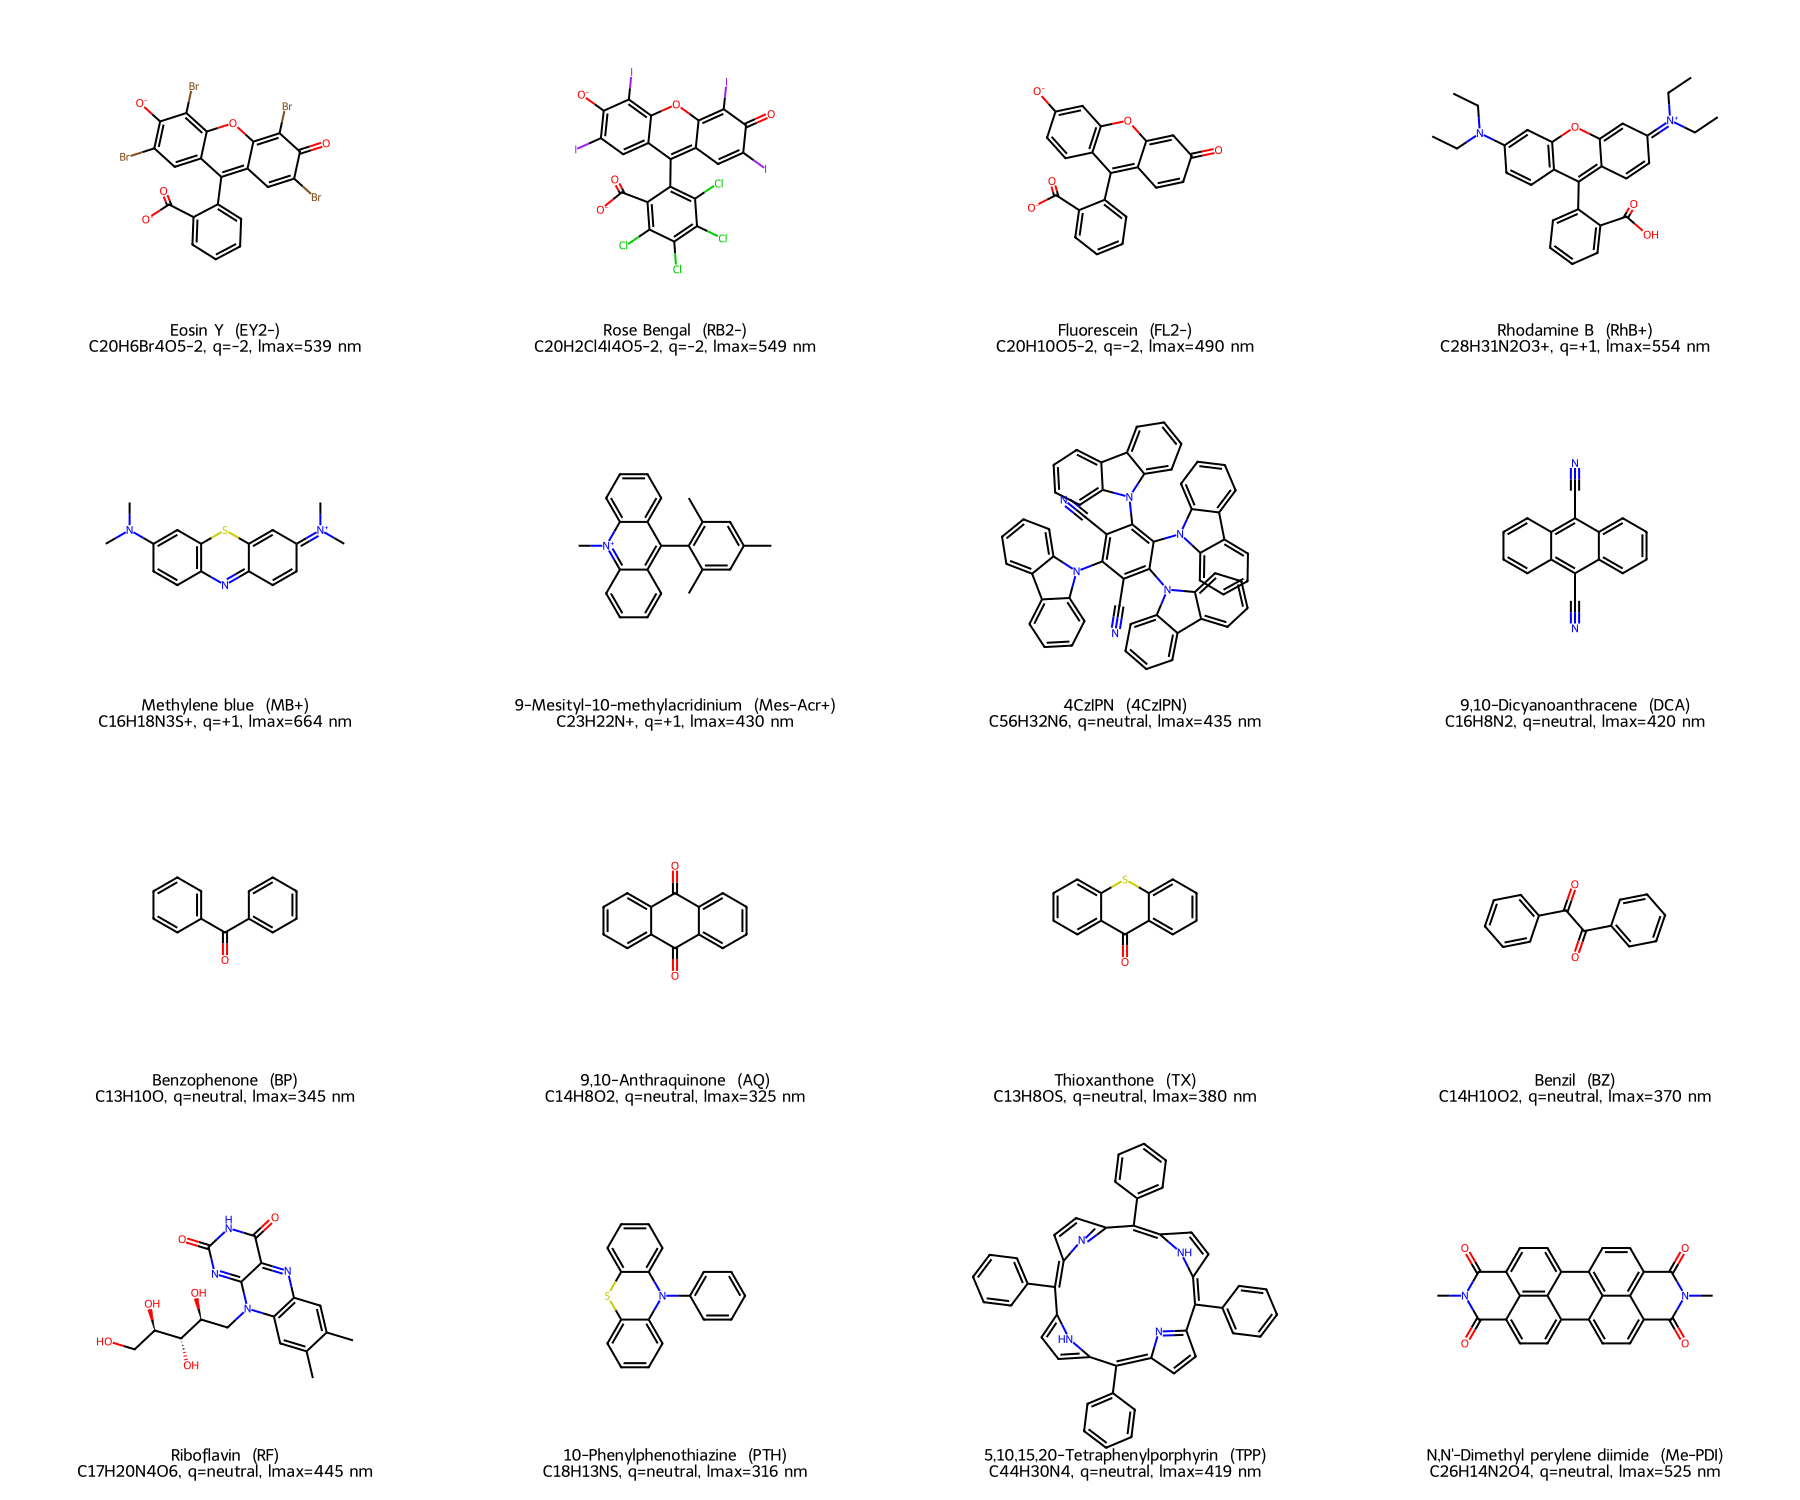
\includegraphics[width=0.72\linewidth]{organic_photocatalysts_grid.png}
\caption*{\small My 16 photocatalysts. The first thing I check now is the little charge signs.}
\end{figure}

\begin{aha}
The ``same'' dye isn't one molecule. Eosin Y in the bottle is neutral, but in water at working
pH it's the \textbf{dianion} \ce{EY^{2-}}. The colour and redox behaviour belong to the dianion,
so that's what I must compute. Same story for fluorescein and rose bengal (dianions), and
methylene blue, rhodamine B and Mes-Acr$^+$ (cations). The 2D drawing makes these charges visible
at a glance.
\end{aha}

Two RDKit things I didn't know before:
\begin{itemize}
  \item \textbf{SMARTS = a search query for a substructure.} I highlighted the xanthene core and
  suddenly saw that eosin Y, fluorescein, rose bengal and rhodamine B are all the same chromophore
  with different things attached. The \texttt{\textasciitilde} in the pattern means ``any bond''.
  It lets the query match whatever bond orders the SMILES uses (here the xanthene is drawn with
  quinoid bonds, not as plain aromatic rings).
  \item \textbf{Atom indices.} When something says ``atom 12'' I can draw the numbers. The xyz
  file uses the same order, which is how I picked four atoms for a dihedral angle later.
\end{itemize}

\begin{figure}[h]
\centering
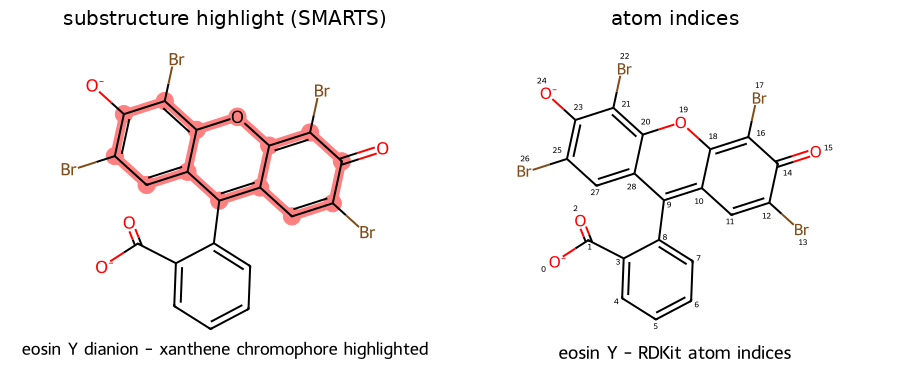
\includegraphics[width=0.72\linewidth]{eosinY_2d_tools.png}
\end{figure}

\textit{Note to self: export SVG not PNG for Overleaf, since it stays sharp.}

%=============================================================================
\section*{2. 3D pictures: the shape matters more than I expected}

How the coordinates are made: SMILES $\to$ add H $\to$ ETKDGv3 (random distance geometry +
torsion preferences from crystal structures) $\to$ MMFF94s force-field clean-up. The final
version tries 8 conformers (30 for floppy molecules) and keeps the lowest.

\q{Why several conformers? Isn't one structure enough?}
For rigid dyes, one is fine. For floppy ones (riboflavin's tail, rhodamine's ethyl groups) a single
random embedding can get stuck in a bad shape. One conformer = one sample, not ``the'' structure.

Styles: \textbf{ball-and-stick} for checking bonds and angles; \textbf{space-filling} for real size
and crowding; \textbf{stick/line} when the molecule is big.

\begin{figure}[h]
\centering
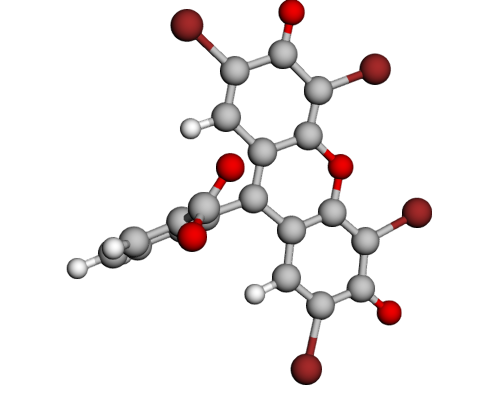
\includegraphics[width=0.33\linewidth]{eosinY_ballstick.png}\hspace{0.05\linewidth}
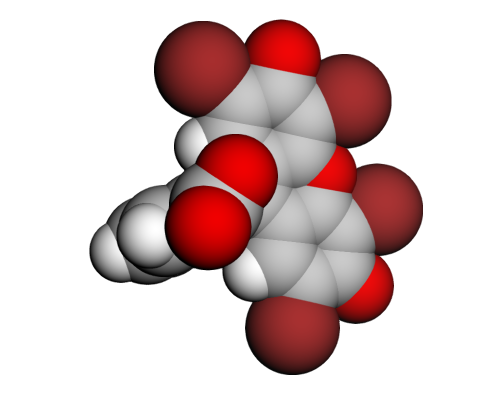
\includegraphics[width=0.33\linewidth]{eosinY_spacefill.png}
\caption*{\small Eosin Y, same coordinates. Left: the benzoate ring is edge-on, i.e.\ twisted.
Right: the four bromines take up a lot of the volume, which I didn't appreciate from 2D.}
\end{figure}

\begin{aha}
Almost every interesting 3D feature in my set is a \textbf{twist}, and twisting controls
\textbf{conjugation}. Two $\pi$ systems at 90$^\circ$ can't share electrons, so they act as
separate pieces.
\begin{itemize}[leftmargin=*]
  \item eosin Y: benzoate $\approx$ perpendicular to the xanthene (I measured \textbf{98.6$^\circ$})
  $\to$ the benzoate hardly affects the colour.
  \item TPP: phenyls twisted out of the porphyrin plane $\to$ the macrocycle is the chromophore.
  \item 4CzIPN: carbazoles twisted $\to$ donor and acceptor decoupled $\to$ TADF / photoredox.
  \item Mes-Acr$^+$: ortho-methyls lock the mesityl orthogonal to the acridinium $\to$ donor and
  acceptor in one molecule but kept apart (comes back in Section 4!).
\end{itemize}
\end{aha}

\begin{figure}[h]
\centering
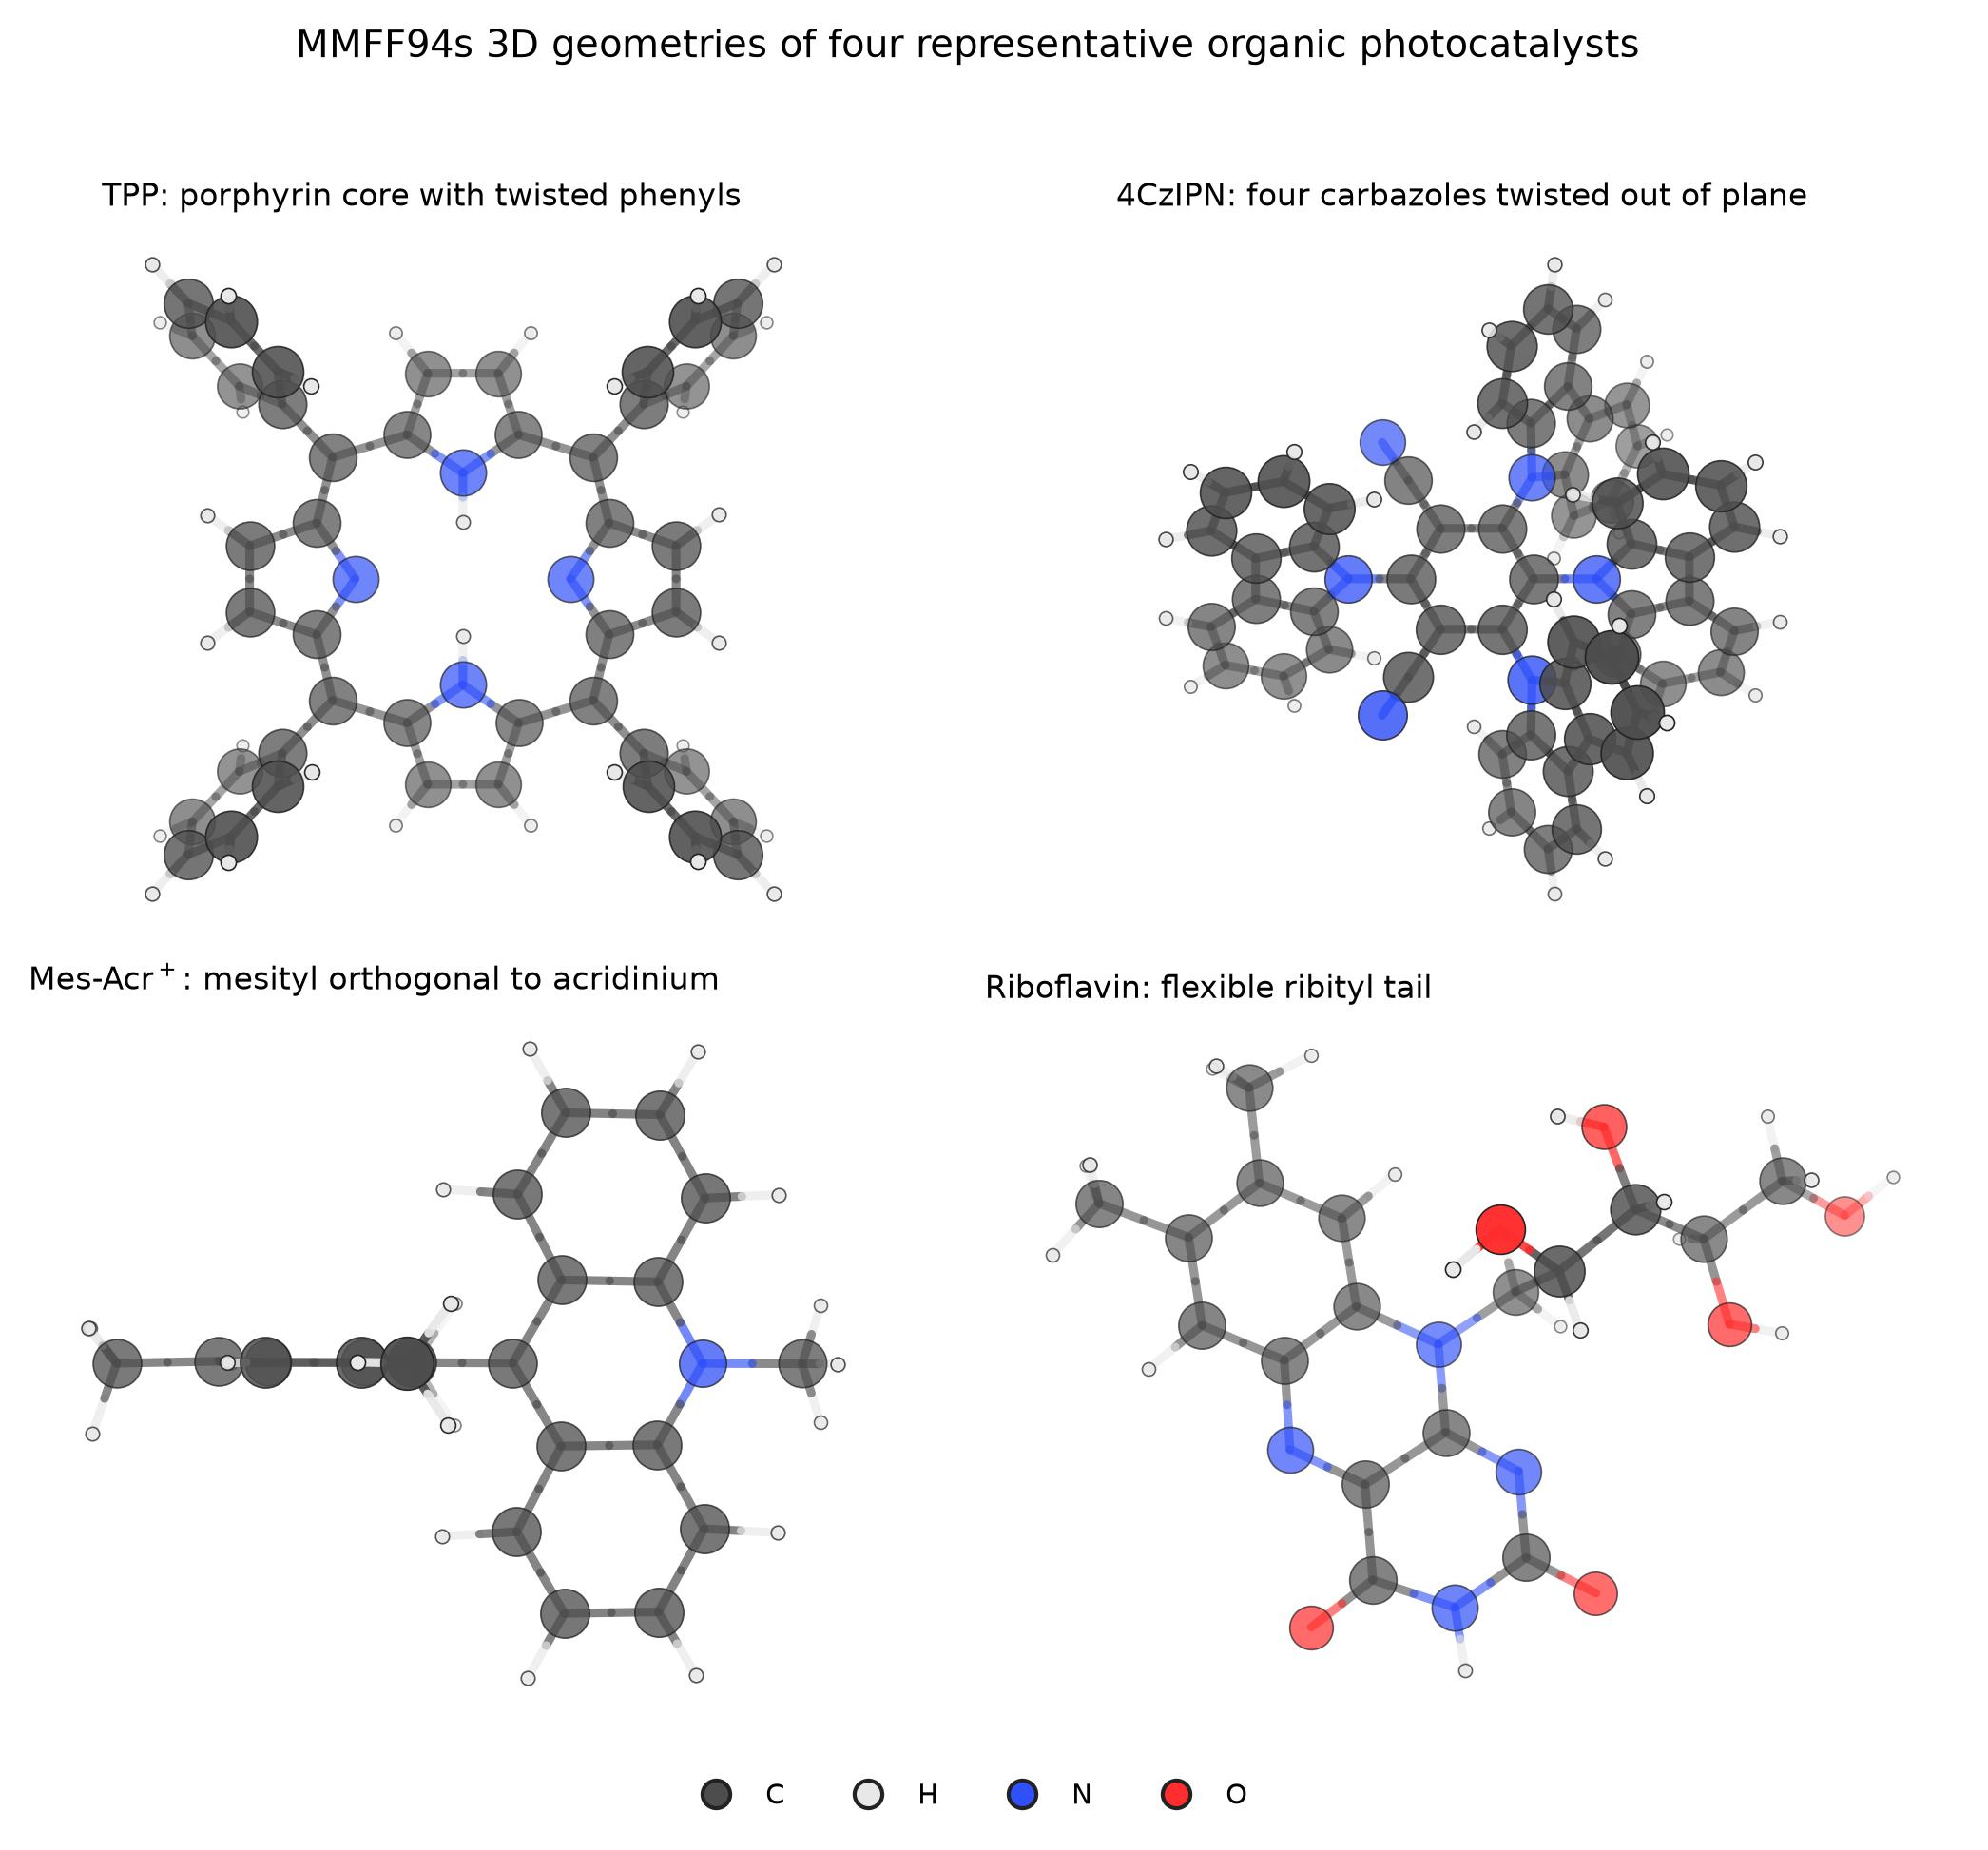
\includegraphics[width=0.62\linewidth]{structures_3d_montage.png}
\end{figure}

\remember{measure, don't eyeball. ``Looks perpendicular'' $\to$ dihedral angle. ``Looks the
same'' $\to$ RMSD.}

%=============================================================================
\section*{3. Overlays: did DFT actually change anything?}

Idea: draw the MMFF start and the DFT result on top of each other.

\begin{figure}[h]
\centering
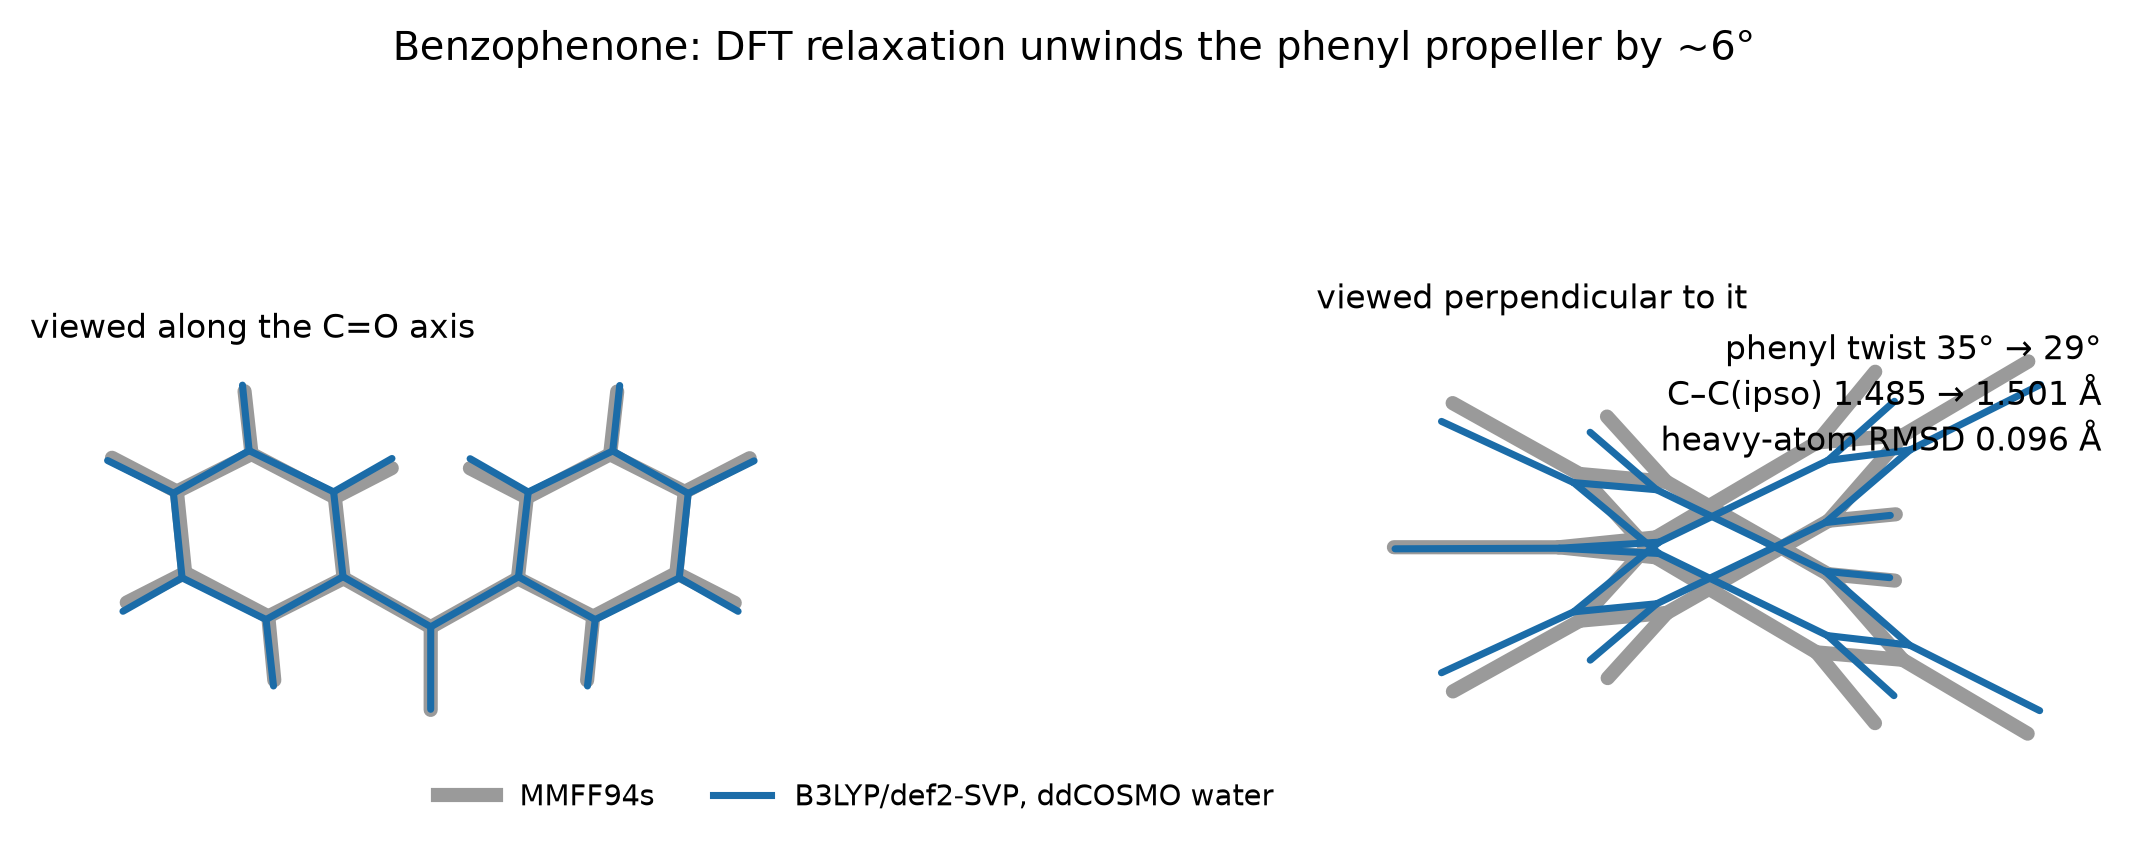
\includegraphics[width=0.9\linewidth]{geomopt_overlay_benzophenone.png}
\end{figure}

\begin{aha}
The left view (along C=O) says ``nothing changed''. The right view shows the phenyl propeller
unwound from 35$^\circ$ to 29$^\circ$. \textbf{The viewing angle can completely hide a change.}
Always look from two directions, and trust the RMSD more than my eyes.
\end{aha}

What the numbers told me:

\begin{center}\small
\begin{tabular}{@{}lccc@{}}
\toprule
& heavy-atom RMSD (\AA) & opt.\ cycles & what it means \\
\midrule
anthraquinone & 0.019 & 15 & rigid $\to$ MMFF basically right \\
thioxanthone & 0.030 & 10 & rigid $\to$ MMFF basically right \\
benzophenone & 0.096 & 11 & 2 rotatable rings $\to$ 5$\times$ worse \\
\bottomrule
\end{tabular}
\end{center}

\begin{oops}
We used these three results to say ``MMFF is good enough'' and then skipped DFT optimisation for
the other 13 molecules. But the three tested were mostly \emph{rigid}, and the one floppy-ish
case was already 5$\times$ worse. The force field is weakest exactly at the torsions between
rings, which is where conjugation is decided. So I can't extend that conclusion to rhodamine B,
riboflavin or the charged dyes without optimising them. \textit{To do.}
\end{oops}

%=============================================================================
\section*{4. Orbitals: the bit I found hardest}

\textbf{How the picture is made:} PySCF evaluates the orbital on a 3D grid $\to$ writes a
\emph{cube file} (plain text; py3Dmol, VESTA, VMD, Avogadro all read it) $\to$ draw two surfaces,
$+$iso and $-$iso, in two colours.

\q{What do the two colours mean?}
Just the sign of the wavefunction. They're \textbf{arbitrary}: $\psi$ and $-\psi$ are the same
orbital. What matters is where the colour \emph{changes}, which is a \textbf{node} (zero amplitude).

\q{How big should the blobs be?}
That's the isovalue, and it's my choice. I drew the same orbital at three values:

\begin{figure}[h]
\centering
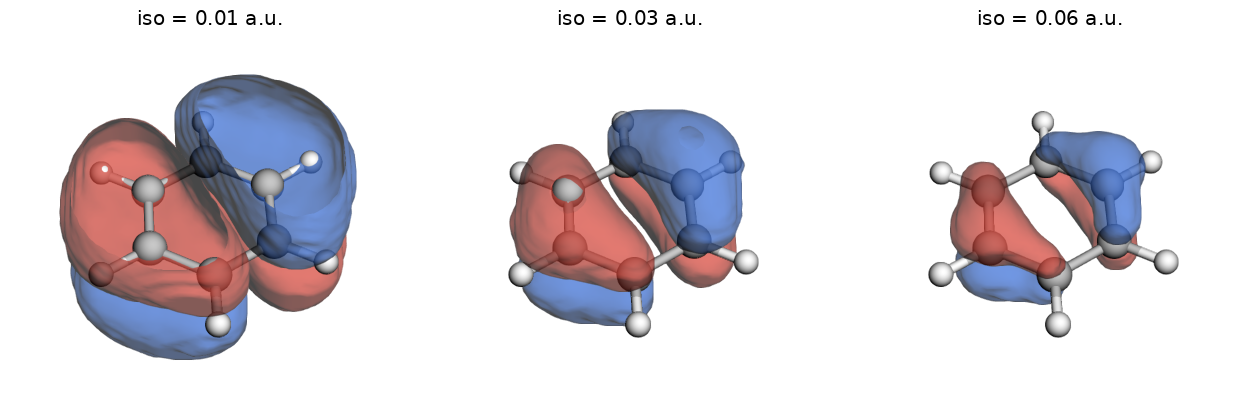
\includegraphics[width=0.85\linewidth]{benzene_isovalue_series.png}
\end{figure}

\begin{aha}
The lobes change size but \textbf{the nodes don't move}. Nodes are physics; lobe size is a
display setting. So: same isovalue for every orbital I compare, and never argue from how
``big'' a lobe looks.
\end{aha}

\textbf{Benzene as a sanity check} (things I can check against the textbook):

\begin{figure}[h]
\centering
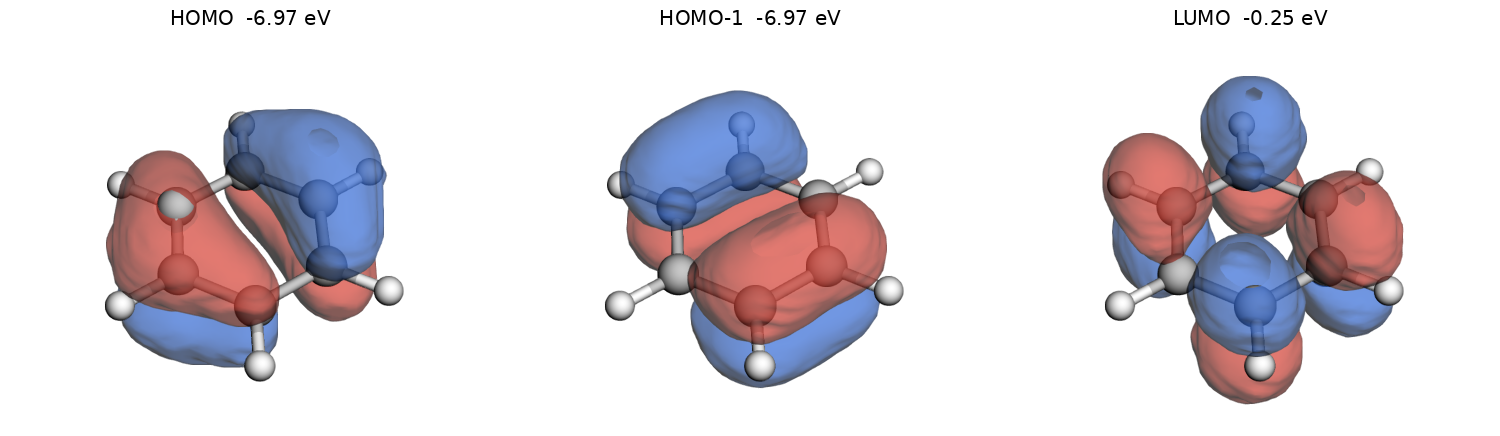
\includegraphics[width=0.75\linewidth]{benzene_frontier.png}
\end{figure}

\begin{itemize}
  \item HOMO and HOMO$-1$ have the \emph{same} energy ($-6.97$ eV): a degenerate pair ($e_{1g}$).
  The program's choice of which way the nodal plane points is arbitrary. \textbf{Don't interpret
  one half of a degenerate pair alone.}
  \item LUMO has two nodal planes vs one for the HOMO. More nodes, higher energy: the
  particle-on-a-ring picture from first year, finally seen directly.
\end{itemize}

\textbf{Then the real catalysts:}

\begin{figure}[h]
\centering
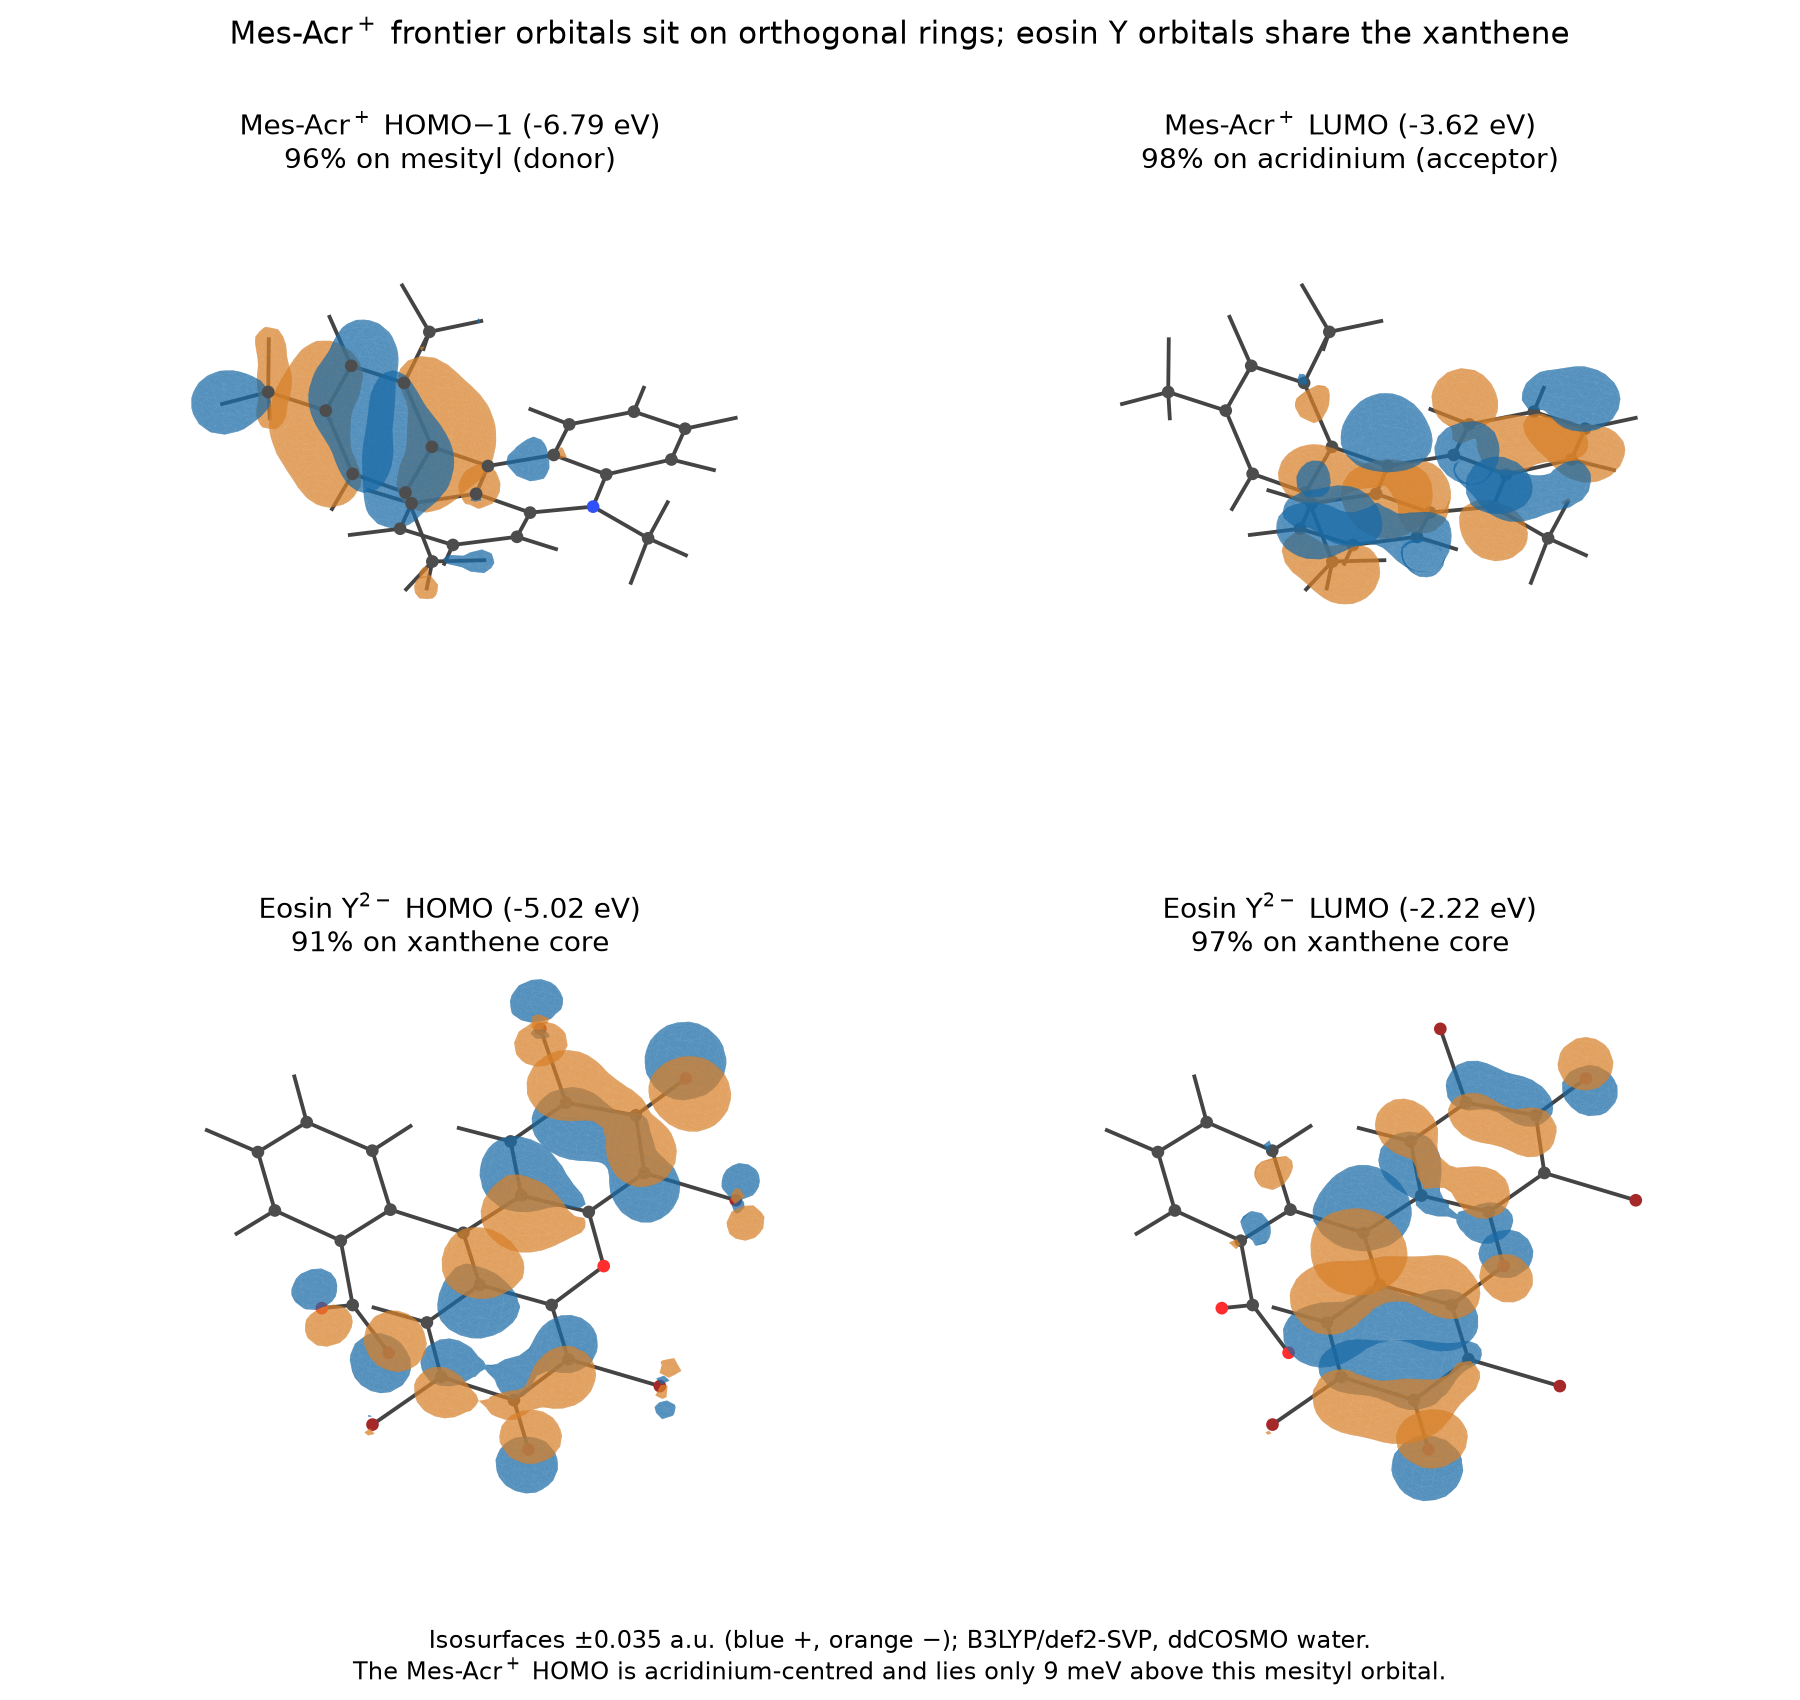
\includegraphics[width=0.6\linewidth]{frontier_orbitals_isosurfaces.png}
\end{figure}

Since a picture depends on the isovalue, we also computed \emph{how much} of each orbital sits on
each fragment (Mulliken populations):

\begin{center}\small
\begin{tabular}{@{}llrl@{}}
\toprule
& orbital & $E$ (eV) & where \\
\midrule
eosin Y$^{2-}$ & HOMO & $-5.02$ & 91\% xanthene \\
 & LUMO & $-2.22$ & 97\% xanthene \\
Mes-Acr$^+$ & HOMO$-2$ & $-6.80$ & $>$99\% mesityl \\
 & HOMO$-1$ & $-6.79$ & 96\% mesityl \\
 & HOMO & $-6.79$ & 99\% acridinium \\
 & LUMO & $-3.62$ & 98\% acridinium \\
\bottomrule
\end{tabular}
\end{center}

\begin{aha}
\textbf{Eosin Y:} electron starts and ends on the xanthene $\to$ \emph{local} $\pi\to\pi^*$.\\
\textbf{Mes-Acr$^+$:} electron can go from the mesityl (donor) to the acridinium (acceptor), two
rings that the 3D picture showed are at 90$^\circ$ $\to$ \emph{charge transfer}. The 3D shape
and the orbital picture are telling the same story. That's the moment it clicked for me.
\end{aha}

\begin{oops}
I was about to write ``the Mes-Acr$^+$ HOMO is on the acridinium''. But the top three occupied
orbitals are within \textbf{13 meV} of each other, far below what B3LYP can resolve. Which one
gets the label ``HOMO'' is basically random at this level. Look at the set, not the label.
\end{oops}

Caveats I need to keep in mind:
\begin{itemize}
  \item Mulliken \% depends on the basis set, so use it for ``91\% vs 10\%'', not ``91\% vs 88\%''.
  \item B3LYP is bad at charge-transfer excitations (Mes-Acr$^+$, 4CzIPN) $\to$ for TDDFT use
  CAM-B3LYP or $\omega$B97X-D.
\end{itemize}

%=============================================================================
\section*{5. The energy-level diagram: the picture that fooled us}

Plotting HOMO/LUMO for all 16 side by side is nice for trends: the HOMO--LUMO gap follows the
lowest absorption band ($r = 0.90$, MAE 0.45 eV). Biggest outlier: benzophenone (+1.37 eV),
because its weak first band is n$\to\pi^*$, not $\pi\to\pi^*$.

\begin{oops}
Our diagram has the H$^+$/H$_2$ and O$_2$/H$_2$O lines drawn across the orbital energies. That
\emph{looks} like it tells me which dyes can split water. It doesn't. From benzene I know
$-$HOMO is $\sim$2 eV off the real ionisation energy with B3LYP, and the HOMO--LUMO gap isn't the
optical gap either. A good correlation means the \emph{trend} is right, not that the absolute
energies are. $\to$ Remove the lines or label them ``qualitative''. Redox needs $\Delta$SCF in
solvent; absorption needs TDDFT.
\end{oops}

%=============================================================================
\section*{6. Practical things I learned the hard way}

\begin{itemize}
  \item \textbf{py3Dmol can't save a PNG on its own}: it needs a browser. Workarounds: a headless
  browser (Playwright), or redraw with matplotlib marching cubes (what Claude Science did). The
  matplotlib ones only roughly handle which surface is in front, so they're schematic. For real
  figures: VESTA or VMD.
  \item \textbf{pyscf-dispersion didn't load on my Mac} $\to$ no D3 correction in these runs.
  Must write that next to every result.
  \item \textbf{Cube files are 3--5 MB each} $\to$ \texttt{*.cube} in \texttt{.gitignore}; they
  regenerate in seconds.
  \item \textbf{AI-written code}: fine, but every script got one test against a known answer
  (benzene, water) before I trusted it on a dye.
\end{itemize}

%=============================================================================
\section*{7. Test myself}

\begin{askme}
\begin{enumerate}[leftmargin=*]
  \item Why is eosin Y computed as \ce{EY^{2-}} and not as the neutral molecule?
  \item What does \texttt{\textasciitilde} mean in a SMARTS pattern, and why use it here?
  \item Why does the benzoate ring in eosin Y barely change its colour?
  \item Why can one viewing direction hide the benzophenone change completely?
  \item If I swap blue and red on an orbital plot, what changes?
  \item The lobes shrink when I raise the isovalue. What stays the same?
  \item Why shouldn't I interpret only the HOMO of benzene?
  \item What links Mes-Acr$^+$'s 3D shape to its orbital picture?
  \item Why is ``the HOMO of Mes-Acr$^+$'' not a meaningful label here?
  \item Why can't I read water-splitting ability off the energy-level diagram?
\end{enumerate}
\end{askme}

\section*{Still unsure / ask Prof.\ Hu}
\begin{itemize}
  \item Is Mulliken OK for fragment \%, or should I use something less basis-dependent
  (Hirshfeld, L\"owdin)?
  \item For the floppy dyes, is a quick xTB conformer search good enough before DFT?
  \item Which isovalue does the group normally use in figures?
\end{itemize}

\section*{Next time I'll\ldots}
\begin{enumerate}
  \item draw 2D and check the charge before anything else;
  \item measure dihedrals / RMSD instead of saying ``looks fine'';
  \item check degenerate or near-degenerate orbitals before naming ``the HOMO'';
  \item use one isovalue throughout and say which;
  \item label every figure with functional / basis / solvent (here: B3LYP/def2-SVP, ddCOSMO
  water, no D3).
\end{enumerate}

\end{document}
